\section{Introduction}

%%Hardware defines the environment within which software operates.  

%% Robots can be very unusual software platforms to develop on, perhaps
%% with novel devices or uncommon processors, frequently assembled by a
%% team stronger in mechanical design than computer science.  In fields
%% such as mobile robotics some standardization can be seen, but in
%% humanoids idiosyncracy is the rule.  Can we avoid being a backwater for
%% software development?  We draw lessons from the free software community
%% and UNIX.


%%%%%%%%%%%%%%%%%%%%%%%%%%
%%% Sorry lorenzo, I'm changing some of this back
%%% where you replaced word ``software'' with ``robotics''.
%%% It just doesn't make as much sense anymore.
%%%     --paulfitz


Robotics development is, in some ways, like natural 
evolution. Consider robot software.
Every piece of software has its niche:
the environmental conditions within which it can be
used.  Within this niche it will grow and change and 
perhaps expand to nearby niches.
%%
Some niches are large (standard PCs),
some are medium-sized (for example robots like 
Khepera~\cite{kephera}, 
Pioneer~\cite{pioneer} and 
AIBO~\cite{aibo} to mention a few), and some are tiny (a newly 
developed humanoid). 
%%
Software evolves quickly as new technologies get proposed 
and hardware changes; if trapped 
in too narrow a niche it tends to become obsolete and die, 
together with the efforts of the developers who have contributed 
to it. 
%%
Robot hardware is subject in turn to the wider commercial and
industrial environment.
%%
In academia, software and hardware designed for robotic 
projects are prone to obsolescence, 
because although graduate students may be 
talented developers they are rarely
experienced and disciplined system engineers.
Also, often the development of a robotic platform is not the main goal 
of the efforts of the people who are working on it but
simply a means to an end.
For such researchers hardware and software development are time 
consuming and tedious tasks that take away time and energy that 
could be better spent doing research. Yet at the same time, the 
design of a robotic platform is a delicate and crucial task that 
cannot be easily delegated to untrained personnel. In research 
laboratories fast changing hardware and lack of human resources 
too often narrow the niche in which robotic platforms live.

%% Software development is, in some ways, like natural 
%% evolution.  Every piece of software has its niche:
%% the environmental conditions within which it can be
%% used.  Within this niche it will grow and change and 
%% perhaps expand to nearby niches.
%% %%
%% Some niches are very large (for example, commercial PCs), some are
%% tiny (a newly developed humanoid). Software evolves quickly 
%% as new technologies get proposed and hardware changes; if trapped 
%% in a too narrow niche it soon tends to become obsolete and die, 
%% together with the efforts of the developers who have contributed 
%% to it. In academia, software written for robotic 
%% projects is prone to obsolescence, 
%% because although graduate students may be 
%% talented programmers they are rarely
%% experienced software engineers.
%% Often also the software is not the main goal of the 
%% efforts of the people who are working on it but
%% simply a means to an end.
%% For such researchers 
%% software development is a time consuming and tedious task that 
%% takes away time and efforts that could be better spent doing 
%% research. Yet at the same time, software development in 
%% robotics is a delicate and crucial task that cannot be easily 
%% delegated to untrained persons. In research laboratories 
%% fast changing hardware and lack of human resources too often 
%% narrow the niche in which software lives.

%
%% Research to provide intelligence to these complicated robots, perhaps
%% of humanoid shape, also suffers. Accumulating knowledge 
%% in the form of working demonstrable systems is plagued by the   
%% difficulty of forming teams, on agreeing on standards, and in 
%% general by the lack of a critical mass in any existing laboratory no 
%% matter the size or funding. 

%% The problem of artificial intelligence seems to be more baffling, and 
%% arguably more difficult, than what originally thought \ref{} and the year 2006 
%% celebrated the $50^{th}$ anniversary of the workshop at Dartmouth College
%% which is unanimously considered the birth of artificial intelligence at 
%% least in some modern sense \ref{}. %Turing had previously considered the problem%
%% A generation of researchers did not manage to make the progress that was
%% certainly hoped for. Significant progress can certainly be made either 
%% because of a breakthrough in our understanding of the problems or through 
%% a slower accumulation of knowledge. Or it can be due to a combination of 
%% these two elements. In addition, the recent paradigmatic shift toward 
%% embodiment seems to require the realization of appropriate robotic 
%% hardware \ref{}. 
%% %Rolf's latest book%
%% This is to say that alternative means have to be found to build a community
%% that can accumulate knowledge and make effective progress. The niche of
%% humanoid robotics and artificial intelligence should be enlarged.

%% In this respect, the parallel with the commercial PC is easily made. 
%% The success of the PC was determined, among other factors, by the definition 
%% of hardware standards that everybody could understand, copy, and reimplement. 
%% From time to time new standards were required (e.g. the ISA bus slowly left
%% space to PCI slots) but the system flourished. A PC of today is the modern 
%% version of the Ship of Theseus\footnote{The Ship of 
%% Theseus -- the mast gets replaced,
%% the planks get replaced, over time everything may get replaced,
%% but it is still in some important sense the same ship (``paradox
%% of identity'')}, everything changed but the PC is still considered
%% a PC. 
%% %

%% Under the hood, the PC is a few orders of magnitude faster and of larger
%% storage capacity. On the software side, the benefit of a common architecture, 
%% allowed creating operating systems and application software consisting of 
%% several millions of lines of code. Without a standard hardware things
%% might have been more difficult.

%% It is clearly difficult to foresee the future of humanoid robotics. It is
%% easier though to imagine a scenario where common standards both in software and
%% hardware will find the fertile soil to flourish when isolated breakthroughs 
%% will happen.

%Research groups that all use a specific robot (Khepera, Pioneer, AIBO,
%...) often form a natural software community.  But each alone is 
%a small subset of robotics.

%Groups developing new robots face obstacles.  There are big barriers
%to software collaboration: differences in sensors, actuators, and
%bodies; differences in processors, operating systems, libraries,
%frameworks, languages, compilers.


%Computer science and PCs operate in a world that has been at least
%partially commodified; research groups in CS do not have to 
%reinvent the operating system for every project they undertake.


%
%In this paper, we are concerned
%about how robotics researchers can avoid being caught in a tiny
%niche, and how to prevent ``genetic isolation'' from setting in,
%where software development is slow and cut-off from the mainstream.
%We want to find a way to avoid this trap, without sacrificing
%the freedom to radically change our hardware, a freedom that
%will be crucial in ``bleeding-edge'' research for years to come.

In this paper, we are concerned
about how robotics researchers can avoid being caught in tiny
niches, and how to prevent ``genetic isolation'' from setting in.
We want to find a way to avoid this trap, without sacrificing
the freedom to radically change hardware and software, a freedom 
that will be crucial in ``bleeding-edge'' research for years to 
come.




\begin{figure}
\centerline{
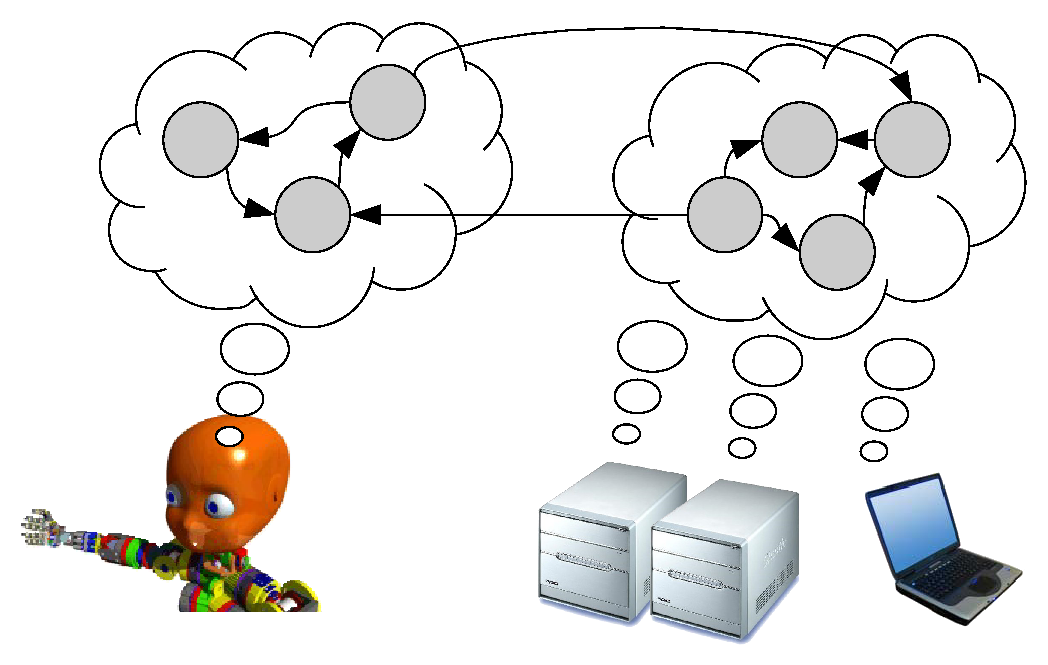
\includegraphics[width=8cm]{fig-nethead}
}
\caption{
%
\label{fig:brain}
%
Our model of a humanoid robot's ``brain''.
We assume a set of processors, some of which may
be on the robot, some of which may not be. We draw no 
distinction; for research purposes, it makes sense to
have off-board processing to do today what robots will
be able to do on-board tomorrow.
%
We assume diversity:
different devices, operating systems, processors, different languages,
libraries, etc. (of course, within our own project we have standards,
but we don't expect everyone using our robot to agree).
%
%We develop methods for interfacing with devices and communicating
%between modules that are useful on any heterogeneous system.
%
We exploit key Free Software tools for smoothing over differences in
operating systems, build systems, and programming languages.
%
We develop YARP, for smoothing over differences in networking,
devices details, and libraries relevant to robotics.
%
%
%We nevertheless require that threads within processes
%on any of these computers be able to communicate easily with each other.
%
%This communication, ideally, should fit well with basic UNIX 
%tools and concepts (although we do not assume the operating systems
%in use are UNIX-based).
%
We release YARP as Free Software
 and use it to support our open robot
platform, the ICub humanoid, whose design will be available under free
and open licensing.
%
}
\end{figure}



From the point of view of software development, the only viable 
solution to these problems is to facilitate 
code reuse both in time (from past to future) and space
(between geographically dispersed people and 
institutions). For projects of a reasonable size this means following
a \emph{modular} approach, where software is ideally divided in 
independent components, that can be developed and maintained 
by different people so that efforts 
are shared among groups having distinct competences. A 
modular software platform is flexible. Obsolete modules are 
removed and substituted for newer ones without 
catastrophic effects. It is difficult to take advantage of code written by 
other people in different contexts unless that code
avoids extraneous constraints 
and dependencies at all levels, from the hardware architecture 
to the development environment and programming language. 
In robotics, dependencies between modules need to be 
minimized also from the point of view of run-time performance; as 
long as resources are available the addition of new 
components should not clash with the 
overall behavior of
existing ones (in terms of throughput, latency, etc).
%
%In 
%particular it should be possible to
%preserve the \emph{timing} of signals 
%irrespective of the number of modules that are running 
%at any given moment in the whole system. 
%
% this would take a while to explain well...
%
%
And from the hardware development point of view, the robotic platform can 
be seen as another factor in the
equation of code reuse. Common hardware, common protocols,
electrical standards, sensors, etc. can certainly make the 
our life easier. As it does for software, modularity 
can play a role in the hardware design too. 

%%% and now I try to close the introduction:
In this paper we describe our efforts to build a modular
humanoid robot platform (see Figure~\ref{fig:brain}). 
We 
describe YARP \cite{metta2006yarp}, an open source library 
that we have developed to support software development on humanoid 
robotics. With YARP we try to facilitate code exchange between researchers, 
especially when this speeds up the time 
it takes to develop a platform and use it for research. We here report 
aspects of YARP that we hope will contribute to longevity and 
interoperability of software developed for robotics. Analogously for
hardware, we describe our efforts to create an open 
robotic platform, the \emph{ICub} that can be shared among several research 
groups worldwide.

Following the Open Source philosophy we make the 
code of our software and hardware available so that other 
researchers can better understand it and have the freedom 
to improve and better adapt it to their needs.
%
%%Our motivation comes from the condition of humanoid robotics 
%%research, but most of this paper is not specific to that field.
%
%
We think it is relevant to any small research group, either academic or
industrial, who wishes to develop novel robots (as opposed to 
build applications on third party robots).  We want to maximize the 
reach of such research groups, being mindful of the fundamental tension 
between providing a consolidated system and giving enough freedom
to change every single part via upgrades and replacements. 
%
%We would
%like to be able to do so both in software and hardware.

%In this sense 
%device-level software development is a very time consuming and tedious 
%task, so the possibility to share code in this context is extremely 
%profitable. 

%Robots with unusual hardware can find themselves initially bereft of
%software, until adaptation occurs.  Therefore robots that take
%advantage of novel hardware may require significant software effort.

%Any given piece of software can operate in a certain set of 
%environments.  Every new robot is a new environment, with some
%overlap with existing ones.  Some software will run there,
%some will not.

%In terms of software, robotic platforms can be quite ``genetically
%isolated'' from the mainstream population of PCs.  

%Humanoid robotics is our passion, but in the grand scheme
%of world-wide software development 

%Big companies built on OSS (e.g. Google)

% this might require a few changes to accomodate for the hardware...
%% New devices come out all the time -- needs to be easy to connect them
%% to existing code.  YARP needs a minimal ``wrapper'' class to match
%% vendor-supplied library with relevant interfaces that capture common
%% capabilities.  YARP encourages separating configuration from source
%% code -- separating the ``plumbing''.  Devices and communications
%% remain distinct concerns.  The goal is to allow collaboration between
%% groups whose robots have different devices and make device changes
%% less painful.  We also want to have the ability to be able to switch
%% from remote use of device to local use and vice versa without pain,
%% without compromising the efficiency of local access.

%% Robots need an analogue of the operating system of a computer, or the
%% nervous system of an animal.  We focus on the key issue of how information
%% travels between processors, sensors, and actuators.

%% We use other key free and open source projects to make
%% our libraries usable in as many environments as possible.  We use the
%% ACE operating system portability layer (but {\it not} the associated
%% implementation of CORBA), the CMake build system, the SWIG wrapper
%% generator.

%% We release our code as free software 
%% \protect\footnote{\tt http://yarp0.sourceforge.net}.

%% We have previously report the basic history of YARP and its 
%% motivations~\cite{metta2006yarp}.
%% We here report aspects of YARP that we hope will contribute to
%% longevity and interoperability.  (((And if we have ICub material,
%% expand scope to include that))).


%% The goal of YARP is to support humanoid robotics, in which a broad 
%% variety of hardware is often employed. In YARP we try to facilitate code 
%% exchange between researchers, especially when this speeds up the time 
%% it takes to develop a platform and use it for research. In this sense 
%% device-level software development is a very time consuming and tedious 
%% task, so the possibility to share code in this context is extremely 
%% profitable. 

%YARP devices consists in a set of \emph{wrapper classes}, 
%which usually link vendor's libraries.... 

